% =============================================================================
%  CS60055 Ubiquitous Computing - Hackathon Challenge 2 presentation
%  Cross-Room Few-Shot Adaptation for WiFi CSI Activity Recognition
%
%  Compile:  cd report && pdflatex slides && pdflatex slides
%  Figures are read from ../results/figures/ (or ./figures/). Any figure that is
%  missing is drawn as a dashed placeholder box, so the deck always compiles.
% =============================================================================
\documentclass[aspectratio=169,10pt]{beamer}

\usetheme{Madrid}
\usefonttheme{serif}
\usepackage[T1]{fontenc}
\usepackage[utf8]{inputenc}
\usepackage{lmodern}
\usepackage{booktabs}
\usepackage{amsmath}
\usepackage{appendixnumberbeamer}
\usepackage{tikz}
\usetikzlibrary{positioning,arrows.meta,calc,shadows,decorations.pathreplacing}
\usepackage[most]{tcolorbox}

% ---- Colours (IIT KGP brown, as in the course slides) -----------------------
\definecolor{kgpbrown}{RGB}{122,74,24}
\definecolor{kgplight}{RGB}{175,148,110}
\definecolor{ourc}{RGB}{196,112,24}
\definecolor{paperc}{RGB}{84,106,138}
\definecolor{goodc}{RGB}{46,125,50}
\definecolor{badc}{RGB}{176,42,42}
% diagram palette (names used throughout the slides)
\colorlet{accent}{kgpbrown}   % Room A / main path
\colorlet{teal}{ourc}         % Task 2 / secondary
\colorlet{violet}{paperc}     % Room B / Task 3
\colorlet{good}{goodc}
\colorlet{bad}{badc}
\colorlet{warn}{kgplight!80!black}
\colorlet{muted}{black!60}
\colorlet{ink}{black}
\colorlet{line}{kgpbrown!35}
\colorlet{cardbg}{kgpbrown!4}
\colorlet{tint}{kgpbrown!9}

\setbeamercolor{palette primary}{bg=kgpbrown,fg=white}
\setbeamercolor{palette secondary}{bg=kgplight,fg=white}
\setbeamercolor{palette tertiary}{bg=kgpbrown,fg=white}
\setbeamercolor{palette quaternary}{bg=kgpbrown,fg=white}
\setbeamercolor{structure}{fg=kgpbrown}
\setbeamercolor{title}{bg=kgpbrown,fg=white}
\setbeamercolor{frametitle}{bg=kgpbrown,fg=white}
\setbeamercolor{block title}{bg=kgpbrown,fg=white}
\setbeamercolor{block body}{bg=kgpbrown!7,fg=black}
\setbeamercolor{block title alerted}{bg=badc,fg=white}
\setbeamercolor{block body alerted}{bg=badc!7,fg=black}
\setbeamercolor{block title example}{bg=goodc,fg=white}
\setbeamercolor{block body example}{bg=goodc!7,fg=black}
\setbeamertemplate{blocks}[rounded][shadow=true]
\setbeamertemplate{navigation symbols}{}
\setbeamertemplate{headline}{}
\setbeamertemplate{itemize items}[circle]

% ---- Helpers ----------------------------------------------------------------
% card: a beamer block whose title bar takes the given colour
\newenvironment{card}[2][accent]{%
  \setbeamercolor{block title}{bg=#1,fg=white}%
  \setbeamercolor{block body}{bg=#1!7,fg=black}%
  \begin{block}{\small #2}\footnotesize}{\end{block}}

% \stat[colour]{big number}{caption}: headline number tile
\newcommand{\stat}[3][accent]{%
  \begin{tcolorbox}[enhanced, colback=#1!8, colframe=#1!60, boxrule=0.6pt, arc=4pt, halign=center,
    top=3pt, bottom=3pt, drop small lifted shadow]
    {\color{#1}\LARGE\bfseries #2}\\[1pt]{\color{muted}\scriptsize #3}
  \end{tcolorbox}}

% \placeholder{width}{height}{text}: dashed box to drop an image into later
\newcommand{\placeholder}[3]{%
  \begin{tikzpicture}
    \node[draw=kgpbrown!60, dashed, very thick, fill=kgpbrown!4, rounded corners=4pt,
          minimum width=#1, minimum height=#2, align=center,
          font=\footnotesize\color{kgpbrown}] {\textbf{[ Image placeholder ]}\\[2pt]#3};
  \end{tikzpicture}}
% \figslot{file}{width}{height}: include a figure if present, else a placeholder
\newcommand{\figslot}[3]{%
  \IfFileExists{../results/figures/#1}{\includegraphics[width=#2,height=#3,keepaspectratio]{../results/figures/#1}}{%
  \IfFileExists{figures/#1}{\includegraphics[width=#2,height=#3,keepaspectratio]{figures/#1}}{%
  \placeholder{#2}{#3}{\texttt{\detokenize{#1}}}}}}

\tikzset{
  blk/.style={draw=kgpbrown, fill=kgpbrown!8, rounded corners=4pt, align=center, font=\scriptsize,
              inner sep=4pt, text=black, drop shadow={opacity=0.25}},
  hot/.style={blk, fill=kgpbrown!18, very thick},
  srcA/.style={blk, fill=ourc!15, draw=ourc},
  srcB/.style={blk, fill=paperc!15, draw=paperc},
  arr/.style={-{Stealth[length=2.2mm]}, thick, draw=kgpbrown},
}

% ---- Title ------------------------------------------------------------------
\title[Cross-Room Few-Shot CSI HAR]{Cross-Room Few-Shot Adaptation}
\subtitle{WiFi CSI Activity Recognition with Very Few Labels}
\author[Team]{\textless Team member names\textgreater \\ {\small \textless Roll numbers\textgreater}}
\institute[IIT Kharagpur]{CS60055 Ubiquitous Computing --- Hackathon Challenge 2\\[2pt]
  Indian Institute of Technology Kharagpur}
\date[Autumn 2026]{Autumn 2026-27}
\titlegraphic{\IfFileExists{kgp_logo.png}{\includegraphics[height=1.3cm]{kgp_logo.png}}{}}

\begin{document}

\begin{frame}
  \titlepage
  \vspace{-6pt}
  \centering{\scriptsize\color{muted} All numbers are validation results on the fixed challenge validation sets.}
\end{frame}

% ===================================================================== problem
\begin{frame}{What we built}
  \vspace{4pt}
  {\color{muted}\small A model trained in one room fails in the next. A new home gets a short setup visit with \emph{a few} labels.}
  \vspace{8pt}

  \begin{columns}[T]
    \column{0.32\textwidth}
    \begin{card}[accent]{Task 1 \textbullet{} Route}
      Which room did this $150\times256$ CSI window come from?\\[3pt]
      {\color{muted}Router for the adapter.}
    \end{card}
    \column{0.32\textwidth}
    \begin{card}[teal]{Task 2 \textbullet{} Learn}
      Learn a CSI encoder \textbf{without any labels} (self-supervised).\\[3pt]
      {\color{muted}Scored by a frozen linear probe.}
    \end{card}
    \column{0.32\textwidth}
    \begin{card}[violet]{Task 3 \textbullet{} Adapt}
      New room: $K$ labelled captures for its \emph{own} activities; shared SIT/STAND/WALK get \textbf{zero} labels.
    \end{card}
  \end{columns}
  \vspace{8pt}

  \begin{columns}[T]
    \column{0.32\textwidth}\stat[accent]{100\%}{room accuracy}
    \column{0.32\textwidth}\stat[teal]{0.946}{joint linear-probe macro-F1}
    \column{0.32\textwidth}\stat[violet]{0.79 / 0.86}{exclusive macro-F1 at $K{=}20$ (A / B)}
  \end{columns}
\end{frame}

% ======================================================================== data
\begin{frame}{Two rooms, two very different archives}
  \begin{columns}[T]
    \column{0.48\textwidth}
    \begin{card}[accent]{Room A \textbullet{} Experiment 2}
      \textbf{1,084 raw \texttt{.pcap}} (934 dev + 150 val)\\
      SIT \textbullet{} STAND \textbullet{} WALK \textbullet{} \textbf{SIT-DOWN \textbullet{} STAND-UP \textbullet{} FALL}\\[3pt]
      {\color{muted}Nexmon packets $\rightarrow$ we decode CSI ourselves.\\
      $\approx$3.9\,s per capture; ``30ms'' is the ping interval.}
    \end{card}
    \column{0.48\textwidth}
    \begin{card}[violet]{Room B \textbullet{} Experiment 3}
      \textbf{1,201 amplitude \texttt{.csv}} ($500\times256$ each)\\
      SIT \textbullet{} STAND \textbullet{} WALK \textbullet{} \textbf{EMPTY \textbullet{} LYING}\\[3pt]
      {\color{muted}Already amplitudes, no timestamps.\\
      Validation: 25/class, seed 42 (we build it).}
    \end{card}
  \end{columns}
  \vspace{8pt}
  \centering
  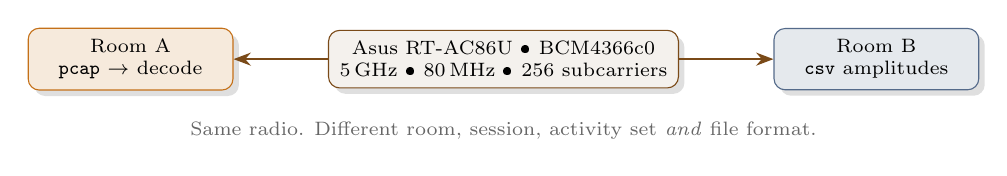
\begin{tikzpicture}[node distance=5mm]
    \node[blk, minimum width=3.2cm] (hw) {Asus RT-AC86U \textbullet{} BCM4366c0\\5\,GHz \textbullet{} 80\,MHz \textbullet{} 256 subcarriers};
    \node[srcA, left=1.2cm of hw, minimum width=2.6cm] (a) {Room A\\\texttt{pcap} $\rightarrow$ decode};
    \node[srcB, right=1.2cm of hw, minimum width=2.6cm] (b) {Room B\\\texttt{csv} amplitudes};
    \draw[arr] (hw) -- (a); \draw[arr] (hw) -- (b);
    \node[below=3mm of hw, muted, font=\scriptsize, align=center] {Same radio. Different room, session, activity set \emph{and} file format.};
  \end{tikzpicture}
\end{frame}

% ===================================================================== CSI 101
\begin{frame}{What is CSI, visually}
  \begin{columns}[T]
    \column{0.52\textwidth}
    \centering
    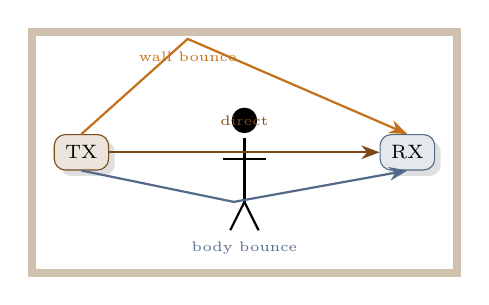
\begin{tikzpicture}[scale=0.9]
      \draw[line, line width=3pt] (0,0) rectangle (6,3.4);
      \node[blk, fill=accent!15, draw=accent] (tx) at (0.7,1.7) {TX};
      \node[blk, fill=violet!15, draw=violet] (rx) at (5.3,1.7) {RX};
      % person
      \draw[ink, thick] (3,1.0) -- (3,1.9); \fill[ink] (3,2.15) circle (0.18);
      \draw[ink, thick] (2.7,1.6) -- (3.3,1.6); \draw[ink, thick] (3,1.0) -- (2.8,0.6); \draw[ink, thick] (3,1.0) -- (3.2,0.6);
      \draw[accent, thick, -{Stealth}] (tx) -- (rx) node[midway, above, font=\tiny, accent, yshift=6pt] {direct};
      \draw[teal, thick, -{Stealth}] (tx.north) -- (2.2,3.3) -- (rx.north);
      \draw[violet, thick, -{Stealth}] (tx.south) -- (2.85,1.0) -- (rx.south);
      \node[font=\tiny, teal] at (2.2,3.05) {wall bounce};
      \node[font=\tiny, violet] at (3.0,0.35) {body bounce};
    \end{tikzpicture}\\[2pt]
    {\color{muted}\scriptsize Copies of the signal add up at RX. When you move, the sum changes.}
    \column{0.46\textwidth}
    \begin{card}[accent]{One frame = one row}
      WiFi splits 80\,MHz into \textbf{256 subcarriers}. For each one the chip reports a complex value $H = I + jQ$.
    \end{card}
    \centering
    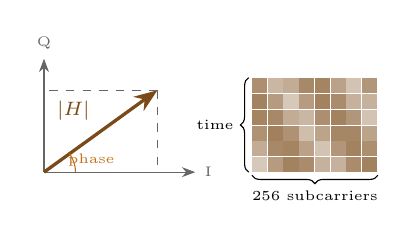
\begin{tikzpicture}[scale=0.8]
      \draw[-{Stealth}, muted] (0,0) -- (2.4,0) node[right, font=\tiny] {I};
      \draw[-{Stealth}, muted] (0,0) -- (0,1.8) node[above, font=\tiny] {Q};
      \draw[accent, very thick, -{Stealth}] (0,0) -- (1.8,1.3) node[midway, above left, font=\scriptsize] {$|H|$};
      \draw[dashed, muted] (1.8,1.3) -- (1.8,0); \draw[dashed, muted] (1.8,1.3) -- (0,1.3);
      \draw[teal] (0.5,0) arc (0:36:0.5); \node[font=\tiny, teal] at (0.75,0.2) {phase};
      % CSI matrix
      \begin{scope}[xshift=3.3cm]
        \foreach \r in {0,...,5} \foreach \c in {0,...,7}
          {\pgfmathtruncatemacro{\shade}{30+40*abs(sin(40*\c+25*\r))}
           \fill[accent!\shade] (0.25*\c,0.25*\r) rectangle ++(0.24,0.24);}
        \draw[decorate, decoration={brace, amplitude=3pt, mirror}] (0,-0.05) -- (2,-0.05)
          node[midway, below=2pt, font=\tiny] {256 subcarriers};
        \draw[decorate, decoration={brace, amplitude=3pt}] (-0.05,0) -- (-0.05,1.5)
          node[midway, left=2pt, font=\tiny] {time};
      \end{scope}
    \end{tikzpicture}\\
    {\color{muted}\scriptsize We use the \textbf{amplitude} $|H|=\sqrt{I^2+Q^2}$.}
  \end{columns}
\end{frame}

% ==================================================================== pipeline
\begin{frame}{End-to-end pipeline}
  \centering
  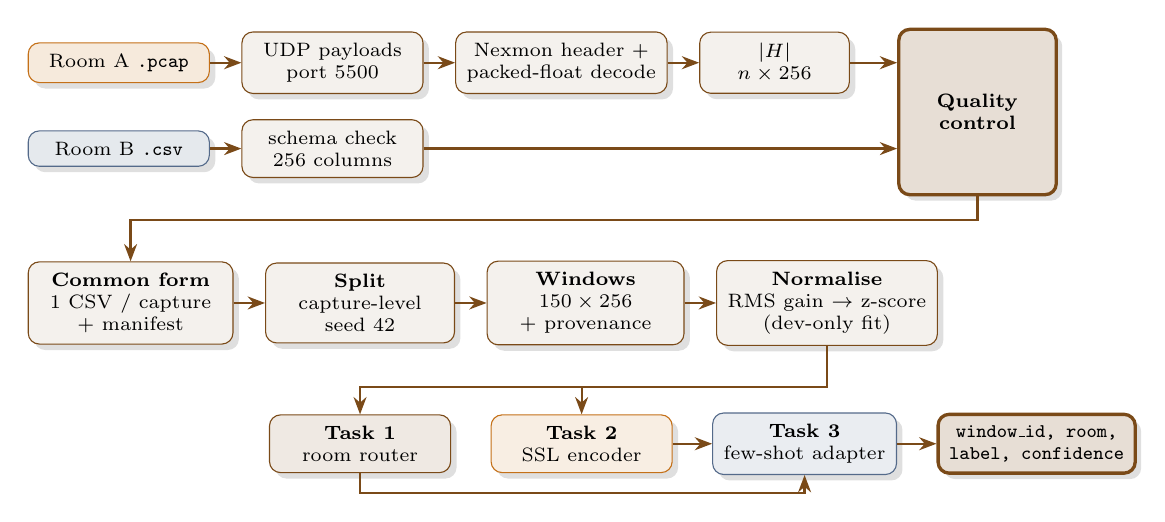
\begin{tikzpicture}[node distance=3.5mm and 4mm, every node/.style={font=\scriptsize}]
    \node[srcA, minimum width=2.3cm] (pcap) {Room A \texttt{.pcap}};
    \node[blk, right=of pcap, minimum width=2.3cm] (udp) {UDP payloads\\port 5500};
    \node[blk, right=of udp, minimum width=2.6cm] (dec) {Nexmon header +\\packed-float decode};
    \node[blk, right=of dec, minimum width=1.9cm] (amp) {$|H|$\\$n\times256$};
    \node[srcB, below=6mm of pcap, minimum width=2.3cm] (csv) {Room B \texttt{.csv}};
    \node[blk, right=of csv, minimum width=2.3cm] (sch) {schema check\\256 columns};
    % QC spans both input rows so both sources enter it from the left
    \node[hot, anchor=north west, minimum height=2.1cm, minimum width=2.0cm] (qc)
      at ($(amp.north east)+(0.6,0.05)$) {\textbf{Quality}\\\textbf{control}};
    \draw[arr] (pcap) -- (udp); \draw[arr] (udp) -- (dec); \draw[arr] (dec) -- (amp);
    \draw[arr] (amp) -- (amp -| qc.west); \draw[arr] (csv) -- (sch); \draw[arr] (sch) -- (sch -| qc.west);

    \node[blk, below=12mm of csv.south west, anchor=north west, minimum width=2.6cm] (cf) {\textbf{Common form}\\1 CSV / capture\\+ manifest};
    \node[blk, right=of cf, minimum width=2.4cm] (sp) {\textbf{Split}\\capture-level\\seed 42};
    \node[blk, right=of sp, minimum width=2.5cm] (win) {\textbf{Windows}\\$150\times256$\\+ provenance};
    \node[blk, right=of win, minimum width=2.7cm] (nrm) {\textbf{Normalise}\\RMS gain $\rightarrow$ z-score\\(dev-only fit)};
    \draw[arr] (qc.south) -- ++(0,-0.3) -| (cf.north);
    \draw[arr] (cf) -- (sp); \draw[arr] (sp) -- (win); \draw[arr] (win) -- (nrm);

    \node[blk, fill=accent!12, draw=accent, below=9mm of sp, minimum width=2.3cm] (t1) {\textbf{Task 1}\\room router};
    \node[blk, fill=teal!12, draw=teal, right=5mm of t1, minimum width=2.3cm] (t2) {\textbf{Task 2}\\SSL encoder};
    \node[blk, fill=violet!12, draw=violet, right=5mm of t2, minimum width=2.3cm] (t3) {\textbf{Task 3}\\few-shot adapter};
    \node[hot, right=5mm of t3, minimum width=2.3cm] (out) {\texttt{window\_id, room,}\\\texttt{label, confidence}};
    \draw[arr] (nrm.south) |- ($(t1.north)+(0,0.35)$) -- (t1.north);
    \draw[arr] ($(t2.north)+(0,0.35)$) -- (t2.north);
    \draw[arr] (t2) -- (t3); \draw[arr] (t1.south) -- ++(0,-0.25) -| (t3.south); \draw[arr] (t3) -- (out);
  \end{tikzpicture}
  \vspace{6pt}

  {\color{muted}\scriptsize After QC both rooms share \emph{one} code path. Every window records its capture, rows and config hash.}
\end{frame}

% ==================================================================== decoding
\begin{frame}{Decoding Room A: inside one packet}
  \centering
  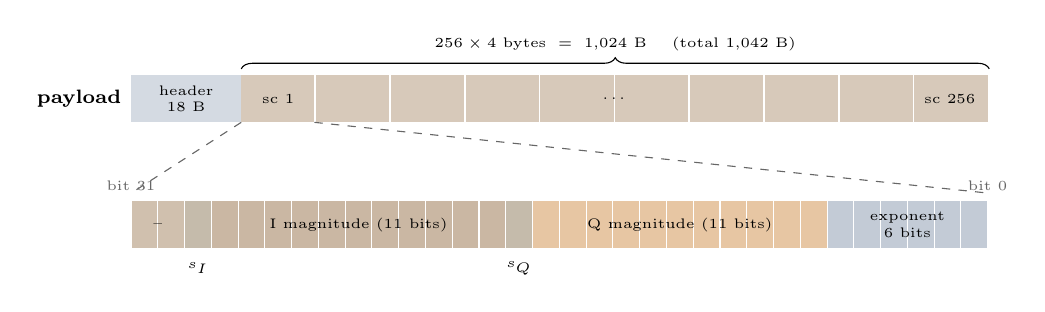
\begin{tikzpicture}[x=1cm, y=1cm]
    % payload bar
    \node[left, font=\scriptsize\bfseries] at (0,0.3) {payload};
    \fill[violet!25] (0,0) rectangle (1.4,0.6); \node[font=\tiny, align=center] at (0.7,0.3) {header\\18 B};
    \foreach \i in {0,...,9} {\fill[accent!30] (1.4+0.95*\i,0) rectangle ++(0.93,0.6);}
    \node[font=\tiny] at (1.87,0.3) {sc 1}; \node[font=\tiny] at (6.15,0.3) {\dots}; \node[font=\tiny] at (10.4,0.3) {sc 256};
    \draw[decorate, decoration={brace, amplitude=4pt}] (1.4,0.68) -- (10.9,0.68)
      node[midway, above=3pt, font=\tiny] {$256 \times 4$ bytes \;=\; 1,024 B \quad(total 1,042 B)};
    % zoom
    \draw[muted, dashed] (1.4,0) -- (0,-0.9); \draw[muted, dashed] (2.33,0) -- (10.9,-0.9);
    % 32-bit word
    \begin{scope}[yshift=-1.6cm, x=0.34cm]
      \fill[line] (0,0) rectangle (2,0.6);
      \fill[warn!50] (2,0) rectangle (3,0.6);
      \fill[accent!40] (3,0) rectangle (14,0.6);
      \fill[warn!50] (14,0) rectangle (15,0.6);
      \fill[teal!40] (15,0) rectangle (26,0.6);
      \fill[violet!35] (26,0) rectangle (32,0.6);
      \foreach \b in {0,...,32} \draw[white, thin] (\b,0) -- (\b,0.6);
      \node[font=\tiny] at (1,0.3) {--};
      \node[font=\tiny] at (2.5,-0.25) {$s_I$};
      \node[font=\tiny] at (8.5,0.3) {I magnitude (11 bits)};
      \node[font=\tiny] at (14.5,-0.25) {$s_Q$};
      \node[font=\tiny] at (20.5,0.3) {Q magnitude (11 bits)};
      \node[font=\tiny, align=center] at (29,0.3) {exponent\\6 bits};
      \node[font=\tiny, muted] at (0,0.8) {bit 31}; \node[font=\tiny, muted] at (32,0.8) {bit 0};
    \end{scope}
  \end{tikzpicture}
  \vspace{8pt}

  \begin{columns}[T]
    \column{0.31\textwidth}
    \begin{card}[violet]{Header}
      magic \texttt{0x1111} \textbullet{} RSSI \textbullet{} MAC \textbullet{} sequence no. \textbullet{} core/stream \textbullet{} chanspec \textbullet{} chip
    \end{card}
    \column{0.31\textwidth}
    \begin{card}[accent]{Value}
      $\text{sign}\cdot m \cdot 2^{e}$ for I and Q,\\then per-packet power-of-two autoscale.
    \end{card}
    \column{0.31\textwidth}
    \begin{card}[good]{Sanity check}
      Empty bins found in the data = exactly the 802.11ac layout (DC 0,1,255; guard 123--133).
    \end{card}
  \end{columns}
\end{frame}

% ========================================================================== QC
\begin{frame}{Quality control: 71\% of Room A frames are not 80\,MHz}
  \begin{columns}[T]
    \column{0.44\textwidth}
    \centering
    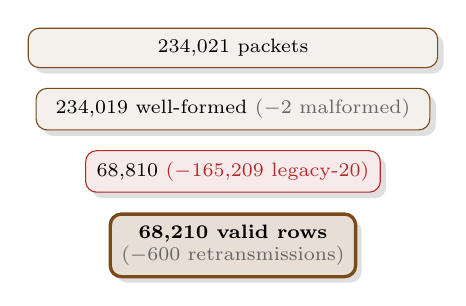
\begin{tikzpicture}[every node/.style={font=\scriptsize, align=center}]
      \node[blk, minimum width=5.2cm] (a) {234,021 packets};
      \node[blk, minimum width=5.0cm, below=2.5mm of a] (b) {234,019 well-formed {\color{muted}($-$2 malformed)}};
      \node[blk, minimum width=3.0cm, below=2.5mm of b, fill=bad!10, draw=bad] (c) {68,810 {\color{bad}($-$165,209 legacy-20)}};
      \node[hot, minimum width=2.9cm, below=2.5mm of c] (d) {\textbf{68,210 valid rows}\\{\color{muted}($-$600 retransmissions)}};
    \end{tikzpicture}\\[4pt]
    {\color{muted}\scriptsize Room B: same rules; legacy-20 removes 7.4\% of rows.}

    \column{0.54\textwidth}
    \begin{card}[bad]{Legacy-20 rule \textbullet{} decided on content}
      \centering
      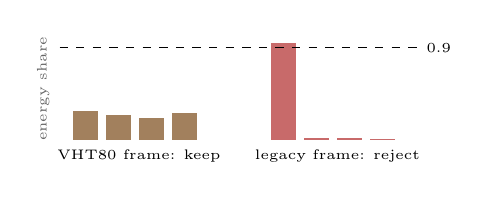
\begin{tikzpicture}[x=0.42cm, y=1.3cm]
        \foreach \v [count=\i] in {0.28,0.24,0.22,0.26}
          {\fill[accent!70] (\i,0) rectangle ++(0.75,\v);}
        \foreach \v [count=\i] in {0.95,0.02,0.02,0.01}
          {\fill[bad!70] (\i+6,0) rectangle ++(0.75,\v);}
        \draw[dashed, ink] (0.6,0.9) -- (11.4,0.9) node[right, font=\tiny] {0.9};
        \node[font=\tiny, below] at (3,0) {VHT80 frame: keep};
        \node[font=\tiny, below] at (9,0) {legacy frame: reject};
        \node[font=\tiny, muted, rotate=90] at (0.1,0.5) {energy share};
      \end{tikzpicture}\\[2pt]
      \raggedright Split the spectrum into four 20\,MHz quarters; reject if one holds $>$90\% of the energy. Bimodal ($\le$0.8 vs $\ge$0.95), so the threshold is safe.\\[2pt]
      {\color{muted}Sequence \texttt{0xFFFF} alone misses 47,306 legacy frames.}
    \end{card}
  \end{columns}
  \vspace{4pt}
  \centering\figslot{fig_qc_examples.png}{0.62\textwidth}{2.1cm}
\end{frame}

% =============================================================== split/window
\begin{frame}{Leakage-safe splits and windows}
  \begin{columns}[T]
    \column{0.48\textwidth}
    \begin{card}[accent]{The capture is the atomic unit}
      \centering
      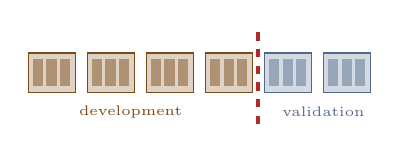
\begin{tikzpicture}[every node/.style={font=\tiny}]
        \foreach \i/\c in {0/accent,1/accent,2/accent,3/accent,4/violet,5/violet}
          {\fill[\c!25, draw=\c] (\i*0.75,0) rectangle ++(0.6,0.5);
           \foreach \w in {0,1,2} \fill[\c!60] (\i*0.75+0.06+\w*0.17,0.08) rectangle ++(0.13,0.34);}
        \node[accent] at (1.3,-0.25) {development};
        \node[violet] at (3.75,-0.25) {validation};
        \draw[bad, very thick, dashed] (2.92,-0.4) -- (2.92,0.8);
      \end{tikzpicture}\\[2pt]
      \raggedright All windows of a capture stay on one side. $K$ counts \emph{captures}, not windows.\\
      Room A: supplied \texttt{validation/}. Room B: 25/class, sorted names, \texttt{Random(42)}.
    \end{card}
    \begin{card}[good]{Fitted on development only}
      normaliser \textbullet{} null-bin mask \textbullet{} router \textbullet{} SSL encoder \textbullet{} alignment \textbullet{} refinement \textbullet{} calibration
    \end{card}

    \column{0.5\textwidth}
    \begin{card}[teal]{Choosing 150 rows}
      \centering
      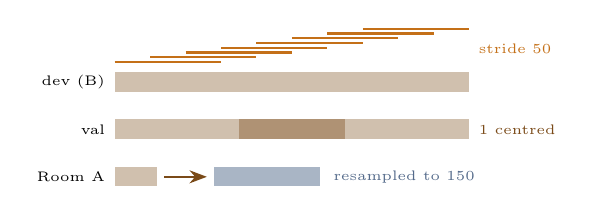
\begin{tikzpicture}[x=0.009cm, every node/.style={font=\tiny}]
        \fill[line] (0,0) rectangle (500,0.25); \node[left] at (0,0.12) {dev (B)};
        \foreach \s [count=\k] in {0,50,...,350}
          {\draw[teal, thick] (\s,0.32+0.06*\k) -- (\s+150,0.32+0.06*\k);}
        \node[right, teal] at (500,0.55) {stride 50};
        \fill[line] (0,-0.6) rectangle (500,-0.35); \node[left] at (0,-0.48) {val};
        \fill[accent!60] (175,-0.6) rectangle (325,-0.35); \node[right, accent] at (500,-0.48) {1 centred};
        \fill[line] (0,-1.2) rectangle (59,-0.95); \node[left] at (0,-1.08) {Room A};
        \draw[arr] (70,-1.08) -- (130,-1.08);
        \fill[violet!50] (140,-1.2) rectangle (290,-0.95); \node[right, violet] at (295,-1.08) {resampled to 150};
      \end{tikzpicture}\\[3pt]
      \raggedright Room A has only 20--118 valid rows. \textbf{Resample, don't pad}: a padding block's length would leak capture length (forbidden metadata).
    \end{card}
    \begin{card}[violet]{Normalise}
      per-row RMS gain {\color{muted}(AGC/autoscale)} $\rightarrow$ per-subcarrier z-score {\color{muted}(pooled)} $\rightarrow$ DC/guard bins set to 0
    \end{card}
  \end{columns}
\end{frame}

% ====================================================================== task 1
\begin{frame}{Task 1: the room is (too) easy to tell}
  \begin{columns}[T]
    \column{0.46\textwidth}
    \centering
    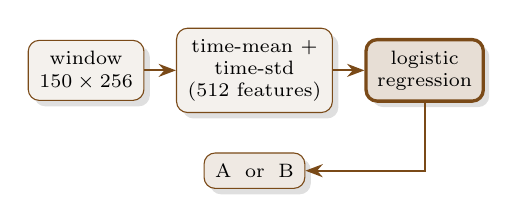
\begin{tikzpicture}[node distance=4mm, every node/.style={font=\scriptsize}]
      \node[blk] (w) {window\\$150\times256$};
      \node[blk, right=of w] (f) {time-mean +\\time-std\\(512 features)};
      \node[hot, right=of f] (lr) {logistic\\regression};
      \node[blk, below=5mm of f, fill=accent!12, draw=accent] (o) {A \;or\; B};
      \draw[arr] (w) -- (f); \draw[arr] (f) -- (lr); \draw[arr] (lr) |- (o);
    \end{tikzpicture}
    \vspace{6pt}

    \begin{columns}
      \column{0.48\linewidth}\stat[accent]{100\%}{274 validation windows}
      \column{0.48\linewidth}\stat[teal]{97.8\%}{from a \emph{single} row}
    \end{columns}
    \vspace{4pt}
    \begin{card}[warn]{Read with care}
      Rooms also differ in noise floor, row-to-row jitter and smoothness. This identifies the \emph{recorded session}, not ``any room''.
    \end{card}
    \column{0.52\textwidth}
    \centering\figslot{fig_room_vs_length.png}{\linewidth}{5.4cm}
  \end{columns}
\end{frame}

% ====================================================================== task 2
\begin{frame}{Task 2: learning without labels (SimCLR)}
  \centering
  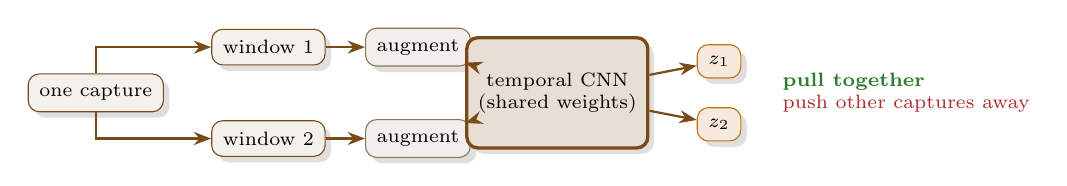
\begin{tikzpicture}[node distance=3mm and 5mm, every node/.style={font=\scriptsize}]
    \node[blk] (cap) {one capture};
    \node[blk, above right=1mm and 6mm of cap] (v1) {window 1};
    \node[blk, below right=1mm and 6mm of cap] (v2) {window 2};
    \node[blk, right=of v1, fill=warn!12, draw=warn] (a1) {augment};
    \node[blk, right=of v2, fill=warn!12, draw=warn] (a2) {augment};
    \coordinate (am) at ($(a1)!0.5!(a2)$);
    \node[hot, right=6mm of am, minimum height=1.4cm, align=center] (enc) {temporal CNN\\(shared weights)};
    \node[blk, right=6mm of enc, yshift=4mm, fill=teal!15, draw=teal] (z1) {$z_1$};
    \node[blk, right=6mm of enc, yshift=-4mm, fill=teal!15, draw=teal] (z2) {$z_2$};
    \coordinate (zm) at ($(z1.east)!0.5!(z2.east)$);
    \node[right=4mm of zm, align=left, text=good] (pull) {\textbf{pull together}\\{\color{bad}push other captures away}};
    \draw[arr] (cap) |- (v1); \draw[arr] (cap) |- (v2);
    \draw[arr] (v1) -- (a1); \draw[arr] (v2) -- (a2);
    \draw[arr] (a1) -- (enc); \draw[arr] (a2) -- (enc);
    \draw[arr] (enc) -- (z1); \draw[arr] (enc) -- (z2);
  \end{tikzpicture}\\[2pt]
  {\color{muted}\scriptsize Augment: crop, gain, spectral tilt, noise, band \& time masking. \textbf{No time reversal}: SIT-DOWN reversed $\approx$ STAND-UP.}
  \vspace{4pt}

  \begin{columns}[T]
    \column{0.5\textwidth}
    \footnotesize
    \begin{tabular}{lccc}
      \toprule
      Linear probe (macro-F1) & Room A & Room B & Joint\\
      \midrule
      \textbf{SSL encoder} & \textbf{0.932} & \textbf{0.992} & \textbf{0.946}\\
      random weights & 0.891 & 0.790 & 0.738\\
      handcrafted & 0.932 & 0.992 & 0.909\\
      \bottomrule
    \end{tabular}\\[4pt]
    {\color{muted}\scriptsize Cross-room probe on shared SIT/STAND/WALK: chance for every representation.}
    \column{0.48\textwidth}
    \centering\figslot{fig_embedding_2d.png}{\linewidth}{3.3cm}
  \end{columns}
\end{frame}

% =============================================================== task 3 method
\begin{frame}{Task 3: the adapter, step by step}
  \centering
  \begin{tikzpicture}[node distance=4mm, every node/.style={font=\scriptsize}]
    \tikzset{step/.style={blk, minimum width=2.45cm, minimum height=1.35cm, text width=2.3cm}}
    \node[step, fill=accent!10, draw=accent] (s1) {\textbf{1 Support}\\$K$ target dev captures per \emph{exclusive} class};
    \node[step, right=of s1, fill=accent!10, draw=accent] (s2) {\textbf{2 Route}\\router picks room $\rightarrow$ stats + label space};
    \node[step, right=of s2, fill=teal!10, draw=teal] (s3) {\textbf{3 Align}\\per-room CORAL whitening (unlabelled dev)};
    \node[step, below=6mm of s1, fill=violet!10, draw=violet] (s4) {\textbf{4 Ensemble}\\prototypes + logistic regression};
    \node[step, right=of s4, fill=violet!10, draw=violet] (s5) {\textbf{5 Refine}\\Sinkhorn soft k-means on target dev};
    \node[step, right=of s5, fill=good!12, draw=good] (s6) {\textbf{6 Calibrate}\\class-balance offsets on target dev};
    \node[hot, right=6mm of s3, yshift=-9.5mm, minimum height=1.2cm, text width=2.2cm, align=center] (o) {label +\\confidence};
    \draw[arr] (s1) -- (s2); \draw[arr] (s2) -- (s3);
    \draw[arr] (s3.south) -- ++(0,-0.15) -| (s4.north);
    \draw[arr] (s4) -- (s5); \draw[arr] (s5) -- (s6); \draw[arr] (s6.east) -| (o.south);
  \end{tikzpicture}
  \vspace{8pt}

  \begin{columns}[T]
    \column{0.48\textwidth}
    \begin{card}[accent]{Source room gives}
      all labels \textbullet{} shared SIT / STAND / WALK learned \emph{only} here
    \end{card}
    \column{0.48\textwidth}
    \begin{card}[bad]{Never used}
      target SIT/STAND/WALK labels \textbullet{} validation windows for any fitting \textbullet{} metadata
    \end{card}
  \end{columns}
\end{frame}

% ============================================================== task 3 results
\begin{frame}{Task 3 results: more labels, better exclusive recognition}
  \begin{columns}[T]
    \column{0.5\textwidth}
    \scriptsize
    \begin{tabular}{llcccc}
      \toprule
      Macro-F1 & Tgt & $K$=1 & 5 & 10 & 20\\
      \midrule
      primary & A & 0.27 & 0.34 & 0.40 & \textbf{0.46}\\
       & B & 0.21 & 0.38 & 0.44 & \textbf{0.43}\\
      \addlinespace
      {\color{good}exclusive} & A & 0.40 & 0.57 & 0.71 & \textbf{0.79}\\
       & B & 0.25 & 0.67 & 0.79 & \textbf{0.86}\\
      \addlinespace
      {\color{bad}shared} & A & 0.14 & 0.10 & 0.08 & 0.14\\
       & B & 0.19 & 0.19 & 0.20 & 0.15\\
      \bottomrule
    \end{tabular}\\[3pt]
    {\color{muted}\scriptsize Mean of 5 support seeds. B$\rightarrow$A = target A.}
    \vspace{4pt}

    \begin{columns}
      \column{0.48\linewidth}\stat[good]{+0.015}{8-cell avg.\ vs prototype-only}
      \column{0.48\linewidth}\stat[accent]{$-$0.16}{without routing ($K$=20, B)}
    \end{columns}
    \column{0.48\textwidth}
    \centering\figslot{fig_label_efficiency.png}{\linewidth}{5.6cm}
  \end{columns}
\end{frame}

% =================================================================== ablations
\begin{frame}{What helps, what does not}
  \begin{columns}[T]
    \column{0.49\textwidth}
    \centering\figslot{fig_routing.png}{\linewidth}{3.0cm}\\[3pt]
    \figslot{fig_ablation.png}{\linewidth}{3.0cm}
    \column{0.49\textwidth}
    \begin{card}[good]{Helps}
      \textbf{Routing} \quad $+$0.14 / $+$0.16 at $K$=20 (A / B)\\
      \textbf{SSL encoder} \quad target B 0.43 vs 0.28 random\\
      \textbf{CORAL} \quad beats diagonal alignment in 8/8 cells\\
      \textbf{Ensemble + calibration} \quad 0.351 $\rightarrow$ 0.366 avg.
    \end{card}
    \begin{card}[warn]{Mixed}
      \textbf{Refinement} \quad helps B at every $K$, hurts A at $K\ge5$\\
      \textbf{Handcrafted} \quad best for A, weak for B
    \end{card}
    \begin{card}[bad]{Does not fix shared classes}
      Removing the static profile lifts WALK recall (0 $\rightarrow$ 0.50 in B) but costs more elsewhere.
    \end{card}
  \end{columns}
\end{frame}

% =================================================================== confusion
\begin{frame}{Confusion at $K=5$: a swap, not a collapse}
  \begin{columns}[T]
    \column{0.52\textwidth}
    \centering\figslot{fig_confusion_K5.png}{\linewidth}{4.0cm}\\[4pt]
    \scriptsize
    \begin{tabular}{lc@{\hspace{10pt}}lc}
      \toprule
      Target A & F1 & Target B & F1\\
      \midrule
      SIT-DOWN & 0.33 $\rightarrow$ \textbf{0.44} & EMPTY & 0.88 $\rightarrow$ \textbf{0.91}\\
      STAND-UP & 0.70 $\rightarrow$ \textbf{0.75} & LYING & 0.50 $\rightarrow$ \textbf{0.56}\\
      FALL & 0.47 $\rightarrow$ \textbf{0.58} & STAND & 0.38 $\rightarrow$ \textbf{0.47}\\
      \bottomrule
    \end{tabular}
    \column{0.46\textwidth}
    \centering
    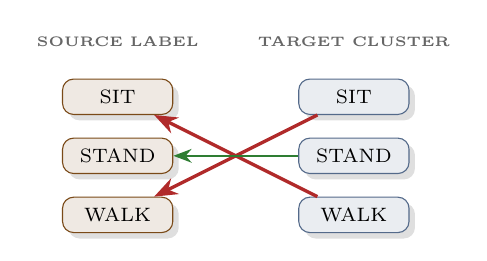
\begin{tikzpicture}[every node/.style={font=\scriptsize}]
      \node[font=\tiny\bfseries, muted] at (0,2.2) {SOURCE LABEL};
      \node[font=\tiny\bfseries, muted] at (3,2.2) {TARGET CLUSTER};
      \foreach \n/\y in {SIT/1.5,STAND/0.75,WALK/0}
        {\node[blk, minimum width=1.4cm, fill=accent!12, draw=accent] (s\n) at (0,\y) {\n};
         \node[blk, minimum width=1.4cm, fill=violet!12, draw=violet] (t\n) at (3,\y) {\n};}
      \draw[bad, very thick, -{Stealth}] (tWALK) -- (sSIT);
      \draw[bad, very thick, -{Stealth}] (tSIT) -- (sWALK);
      \draw[good, thick, -{Stealth}] (tSTAND) -- (sSTAND);
    \end{tikzpicture}\\[4pt]
    \begin{card}[bad]{Why calibration cannot fix it}
      Target WALK $\rightarrow$ SIT (A 18/25, B 14/25); target-B SIT $\rightarrow$ WALK (16/25).\\[2pt]
      Clusters exist but carry the \emph{wrong} source label. Balancing counts cannot un-swap them without target labels.
    \end{card}
  \end{columns}
\end{frame}

% ================================================================== root cause
\begin{frame}{Root cause: the rooms are different measurements}
  \begin{columns}[T]
    \column{0.5\textwidth}
    \begin{card}[violet]{Room B rows are independent snapshots}
      \centering
      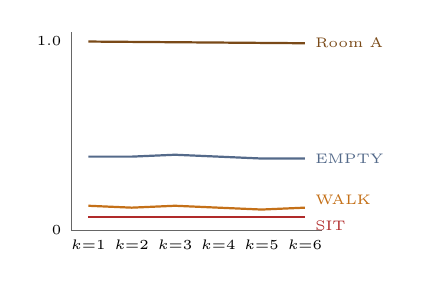
\begin{tikzpicture}[x=0.55cm, y=2.4cm, every node/.style={font=\tiny}]
        \draw[muted] (0.6,0) -- (6.4,0); \draw[muted] (0.6,0) -- (0.6,1.05);
        \foreach \k in {1,...,6} \node[below] at (\k,0) {$k$=\k};
        \node[left] at (0.6,1) {1.0}; \node[left] at (0.6,0) {0};
        \draw[accent, thick] (1,0.999) -- (6,0.99) node[right] {Room A};
        \draw[violet, thick] (1,0.39) -- (2,0.39) -- (3,0.40) -- (4,0.39) -- (5,0.38) -- (6,0.38) node[right] {EMPTY};
        \draw[teal, thick] (1,0.13) -- (2,0.12) -- (3,0.13) -- (4,0.12) -- (5,0.11) -- (6,0.12) node[right, yshift=3pt] {WALK};
        \draw[bad, thick] (1,0.07) -- (6,0.07) node[right, yshift=-3pt] {SIT};
      \end{tikzpicture}\\[2pt]
      \raggedright Correlation of row $i$ vs $i{+}k$ is \textbf{flat}: no interleaved streams, no motion in row order.
    \end{card}
    \column{0.48\textwidth}
    \begin{card}[accent]{Three causes}
      \textbf{1 Measurement:} ``high variation'' means WALK in A but SIT/STAND in B $\Rightarrow$ the swap.\\[2pt]
      \textbf{2 Location:} Room A activities were done in different zones; the static profile encodes \emph{where}.\\[2pt]
      \textbf{3 Session:} rooms recorded separately; alignment removes room shifts, not class-specific ones.
    \end{card}
    \begin{card}[good]{What works}
      Exclusive activities from few captures \textbullet{} routing \textbullet{} SSL for target B
    \end{card}
  \end{columns}
\end{frame}

% ========================================================================= demo
\begin{frame}{Reproduce it and run an episode}
  \begin{columns}[T]
    \column{0.5\textwidth}
    \begin{card}[accent]{Full pipeline \textbullet{} $\approx$70 min on a laptop CPU}
      \ttfamily\scriptsize
      python run\_all.py\\
      {\color{muted}\# inspect$\rightarrow$dataset$\rightarrow$ssl$\rightarrow$task1$\rightarrow$task2$\rightarrow$task3$\rightarrow$figures}
    \end{card}
    \begin{card}[teal]{Live episode}
      \ttfamily\scriptsize
      python run\_episode.py --episode DIR\\
      \phantom{python} [--target-room A|B]\\[3pt]
      {\color{muted}\rmfamily DIR/query/ \textbullet{} .pcap / .csv / .npy\\
      DIR/support/<ACTIVITY>/ (optional)}
    \end{card}
    \column{0.48\textwidth}
    \centering
    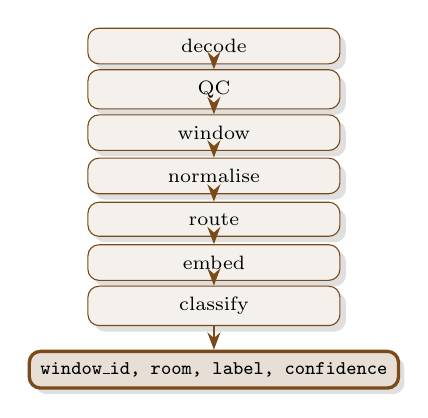
\begin{tikzpicture}[node distance=2.2mm, every node/.style={font=\scriptsize}]
      \foreach \stage [count=\i] in {decode,QC,window,normalise,route,embed,classify}
        {\node[blk, minimum width=3.2cm] (n\i) at (0,-0.55*\i) {\stage};}
      \foreach \i [evaluate=\i as \j using int(\i+1)] in {1,...,6} \draw[arr] (n\i) -- (n\j);
      \node[hot, below=3mm of n7, minimum width=3.2cm] (csv) {\texttt{window\_id, room, label, confidence}};
      \draw[arr] (n7) -- (csv);
    \end{tikzpicture}\\[3pt]
    {\color{muted}\scriptsize Same code path as development and validation data.}
  \end{columns}
\end{frame}

% ==================================================================== takeaways
\begin{frame}{Takeaways}
  \begin{columns}[T]
    \column{0.32\textwidth}
    \begin{card}[accent]{Data engineering}
      Own BCM4366c0 decoder. Found and removed 71\% legacy-20\,MHz frames by \emph{content}. Leakage-safe, auditable windows.
    \end{card}
    \column{0.32\textwidth}
    \begin{card}[teal]{Representation}
      Label-free SimCLR encoder beats random weights by $+$0.20 on Room B and matches handcrafted features.
    \end{card}
    \column{0.32\textwidth}
    \begin{card}[violet]{Adaptation}
      Routing + CORAL + ensemble + calibration: exclusive macro-F1 up to 0.79 (A) / 0.86 (B) at $K$=20.
    \end{card}
  \end{columns}
  \vspace{6pt}
  \begin{card}[bad]{Honest limitation}
    Shared SIT/STAND/WALK stay at chance: a label swap caused by measurement and location differences, which no label-free method can resolve. Validation guided design choices; results are capture-disjoint, not subject-disjoint.
  \end{card}
  \vspace{6pt}
  \begin{columns}[T]
    \column{0.48\textwidth}
    {\scriptsize\color{muted}\textbf{Contribution:} \textless who did what\textgreater}
    \column{0.48\textwidth}
    {\scriptsize\color{muted}\textbf{AI use:} developed with Claude (Anthropic) via Claude Code; see the report's disclosure section.}
  \end{columns}
\end{frame}

\begin{frame}
  \vfill\centering
  {\color{kgpbrown}\Huge\bfseries Thank you}\par\vspace{10pt}
  {\color{kgpbrown}\rule{3cm}{1.5pt}}\par\vspace{10pt}
  {\large Questions?}\par\vspace{4pt}
  {\small\color{muted} Live demo: \texttt{python run\_episode.py --episode DIR}}
  \vfill
\end{frame}

\end{document}
